%%%%%%%%%%%%%%%%%%%%%%%%%%%%%%%%%%%%%%%%%%%%%%%%%%%%%%
% A Beamer template for Ritsumeikan University       %
% Author: Ming-Hao Xu (Xu Minghao)                   %
% Date:   April 2022.                                %
% LPPL Licensed.                                     %
%%%%%%%%%%%%%%%%%%%%%%%%%%%%%%%%%%%%%%%%%%%%%%%%%%%%%%

\documentclass{beamer}
\usepackage{hyperref}

\usepackage[UTF8]{ctex}
\usepackage[T1]{fontenc}

% other packages
\usepackage{latexsym,amsmath,xcolor,multicol,booktabs,calligra}
\usepackage{graphicx,pstricks,listings,stackengine}
\usefonttheme[onlymath]{serif}

% dummy text; remove it when working on this template
\usepackage{lipsum}

\author{Ebola}
\title{字符串进阶:AC自动机}
\institute{
    Institute of Mathematics, \\
    Zhejiang University.
}
\date{Jan, 2024}
\usepackage{Ritsumeikan}

% defs
\def\cmd#1{\texttt{\color{red}\footnotesize $\backslash$#1}}
\def\env#1{\texttt{\color{blue}\footnotesize #1}}
\definecolor{deepblue}{rgb}{0,0,0.5}
\definecolor{deepred}{rgb}{0.6,0,0}
\definecolor{deepgreen}{rgb}{0,0.5,0}
\definecolor{halfgray}{gray}{0.55}

\lstset{
    basicstyle=\ttfamily\tiny,
    keywordstyle=\bfseries\color{deepblue},
    emphstyle=\ttfamily\color{deepred},    % Custom highlighting style
    stringstyle=\color{deepgreen},
    numbers=left,
    numberstyle=\small\color{halfgray},
    rulesepcolor=\color{red!20!green!20!blue!20},
    frame=shadowbox,
}


\begin{document}

\begin{frame}
    \titlepage
\end{frame}

\begin{frame}
    \tableofcontents[sectionstyle=show,subsectionstyle=show/shaded/hide,subsubsectionstyle=show/shaded/hide]
\end{frame}

\section{基础回顾}

\begin{frame}{字典树(Trie)}
    \small

    字典树把所有的字符串存储在一棵树中,
    可以方便地查询所有的前缀。

    \vspace{1em}
    我们来回顾一下字典树模板题。
\end{frame}

\begin{frame}[fragile]{字典树(Trie)}
    \small

    插入操作
    \begin{lstlisting}[language=c++]
int mapping(char c){
    if(c>='A' && c<='Z') return c-'A';
    else return c-'a'+26;
}
void insert(char s[]){
    int n = strlen(s+1);
    int cur = 0;
    sz[0]++;
    for(int i = 1; i <= n; i++){
        int j = mapping(s[i]);
        if(ch[cur][j]==0){
            ch[cur][j] = tot;
            tot++;
        }
        cur = ch[cur][j];
        sz[cur]++;
    }
}
    \end{lstlisting}
\end{frame}

\begin{frame}[fragile]{字典树(Trie)}
    \small

    查询操作
    \begin{lstlisting}[language=c++]
int query(char s[]){
    int cur = 0;
    int n = strlen(s+1);
    for(int i = 1; i <= n; i++){
        int j = mapping(s[i]);
        if(ch[cur][j]==0) return 0;
        cur = ch[cur][j];
    }
    return sz[cur];
}
    \end{lstlisting}
\end{frame}

\begin{frame}{最大异或和问题}
    \small

    最大异或和问题是 Trie 的一个经典应用。

    \vspace{1em}
    给定 $n\;(\leq 10^5)$ 个数,所有数均不超过 $2^{31}-1$.
    从中选两个数,使它们异或起来最大。 
\end{frame}

\begin{frame}{最大异或和问题}
    \small

    把所有的数都转化为 $31$ 位二进制数,高位不足则补零,
    然后把二进制数当成字符串插入进 Trie 中。

    \vspace{1em}\pause
    现在,我们枚举 $x=a_i\;(i=1,...,n)$,来找一个数 $a_j$,使它和 $x$ 异或起来最大。

    \vspace{1em}\pause
    从高位到低位贪心,尽可能让异或和的高位为 $1$。例如:
    如果 $x$ 最高位是 $0$,那么我们希望选出的 $a_j$ 最高位是 $1$,
    这样异或起来最高位才会是 $1$,因此我们第一步从 Trie 的根节点
    往 $1$ 的方向走。
\end{frame}

\begin{frame}[fragile]{最大异或和问题}
    \small

    总之,如果 $x$ 的第 $k$ 位是 $x_{k}$,那么这一步就尽量往 $x_{k}\;\text{xor}\; 1$
    方向走,除非 Trie 不存在对应的分支,此时不得不往 $x_{k}$ 走。
    最后代码像这样:
    \begin{lstlisting}[language=c++]
int query(int x){
    int cur = 0;
    const int n = 31;
    for(int i = 1; i <= n; i++){
        int j = (x >> (31-i)) & 1;
        if(ch[cur][j^1]==0) cur = ch[cur][j];
        else cur = ch[cur][j^1];
    }
    return val[cur];
}
    \end{lstlisting}
\end{frame}

\begin{frame}[fragile]{第 k 大异或和问题}
    \small

    如果想对于给定的 $x$,找到一个 $a_i$,使 $x\oplus a_i$ 是
    $x\oplus a_1,...,x\oplus a_n$ 中第 $k$ 大的数,应该如何写?

    \pause
    \begin{lstlisting}[language=c++]
int query(int x, int k)
{
    int o=1;
    int res=0;
    for(int i=31;i>=0;i--)
    {
        int j=(x>>i)&1;
        if(sz[ch[o][j^1]]>=k) o=ch[o][j^1],res|=1u<<i;
        else k-=sz[ch[o][j^1]],o=ch[o][j];
    }
    return res;
}
    \end{lstlisting}
\end{frame}

\begin{frame}[fragile]{[十二省联考 2019] 异或粽子}
    \small

    给定 $n\;(\leq 5\times 10^5)$ 个数 $a_1,...,a_n$,选一个区间 $[l,r]$,将 $a_l,...,a_r$ 全部异或起来,
    得到这个区间的权值。求权值前 $m\;(\leq 2\times 10^5)$ 大的区间权值之和。
\end{frame}

\begin{frame}[fragile]{[十二省联考 2019] 异或粽子}
    \small

    令 $b_i=a_1\oplus...\oplus a_i$,那么 $a_l\oplus...\oplus a_r=b_{l-1}\oplus b_r$,转化为两个数的异或,
    可以用 Trie 解决。

    \vspace{1em}\pause
    具体地,先把 $b_0,...,b_n$ 的二进制插入 Trie 中。
    接下来对每个 $b_i$ 找到一个 $b_j$ 使它和 $b_i$ 异或起来最大。

    \vspace{1em}\pause
    将这些值存进一个优先队列中。每次从优先队列取出最大的异或和,弹出,
    如果它是 $b_i$ 和其它数的异或和中第 $k$ 大的,
    就找到 $b_i$ 和其它数的异或和中第 $k+1$ 大的加入优先队列。
    不断重复,直到弹出的数达到 $2m$ 个为止,最后答案要除以 $2$. (为什么?)
\end{frame}

\section{AC自动机}

\begin{frame}[fragile]{基本概念}
    \small
    AC自动机 = 字典树 + fail数组

    \vspace{1em}
    对所有模式串建立字典树,根节点为 $0$ 号。
    
    \vspace{1em}\pause
    设 $p$ 是字典树上的一个节点,从根节点到 $p$ 的路径上所有的字母拼起来一定是某个模式串的前缀,我们记这个前缀为 $S_p$,我们说它是 $p$ 代表的字符串
    
    \vspace{1em}\pause
    \verb|fail[p]| 是字典树的一个节点,而且它代表的前缀也是 $S_p$ 的后缀,并且是最长的那个。\pause 用数学语言就是:
    
    \begin{equation*}
        \mathcal{F}(p)=\{q \;|\; q \text{是节点,满足} q\neq p \text{,且} S_q \text{是} S_p \text{的后缀}\}
    \end{equation*}
    
    \begin{equation*}
        fail[p]\in\mathcal{F}(p),\quad \text{且} \;|S_{fail[p]}| = \max_{q\in \mathcal{F}(p)} |S_q|
    \end{equation*}
    
    \pause 特别地,如果 $\mathcal{F}(p)=\varnothing$,那么 $fail[p]=0$。
\end{frame}

\begin{frame}[fragile]{fail 树}
    \small
    如果把每个节点 $p$ 向 $fail[p]$ 连一条蓝色的边,
    我们会发现,所有蓝色的边构成一棵树,其中 $p$ 的父亲是 $fail[p]$.

    \begin{figure}[H]
        \centering
        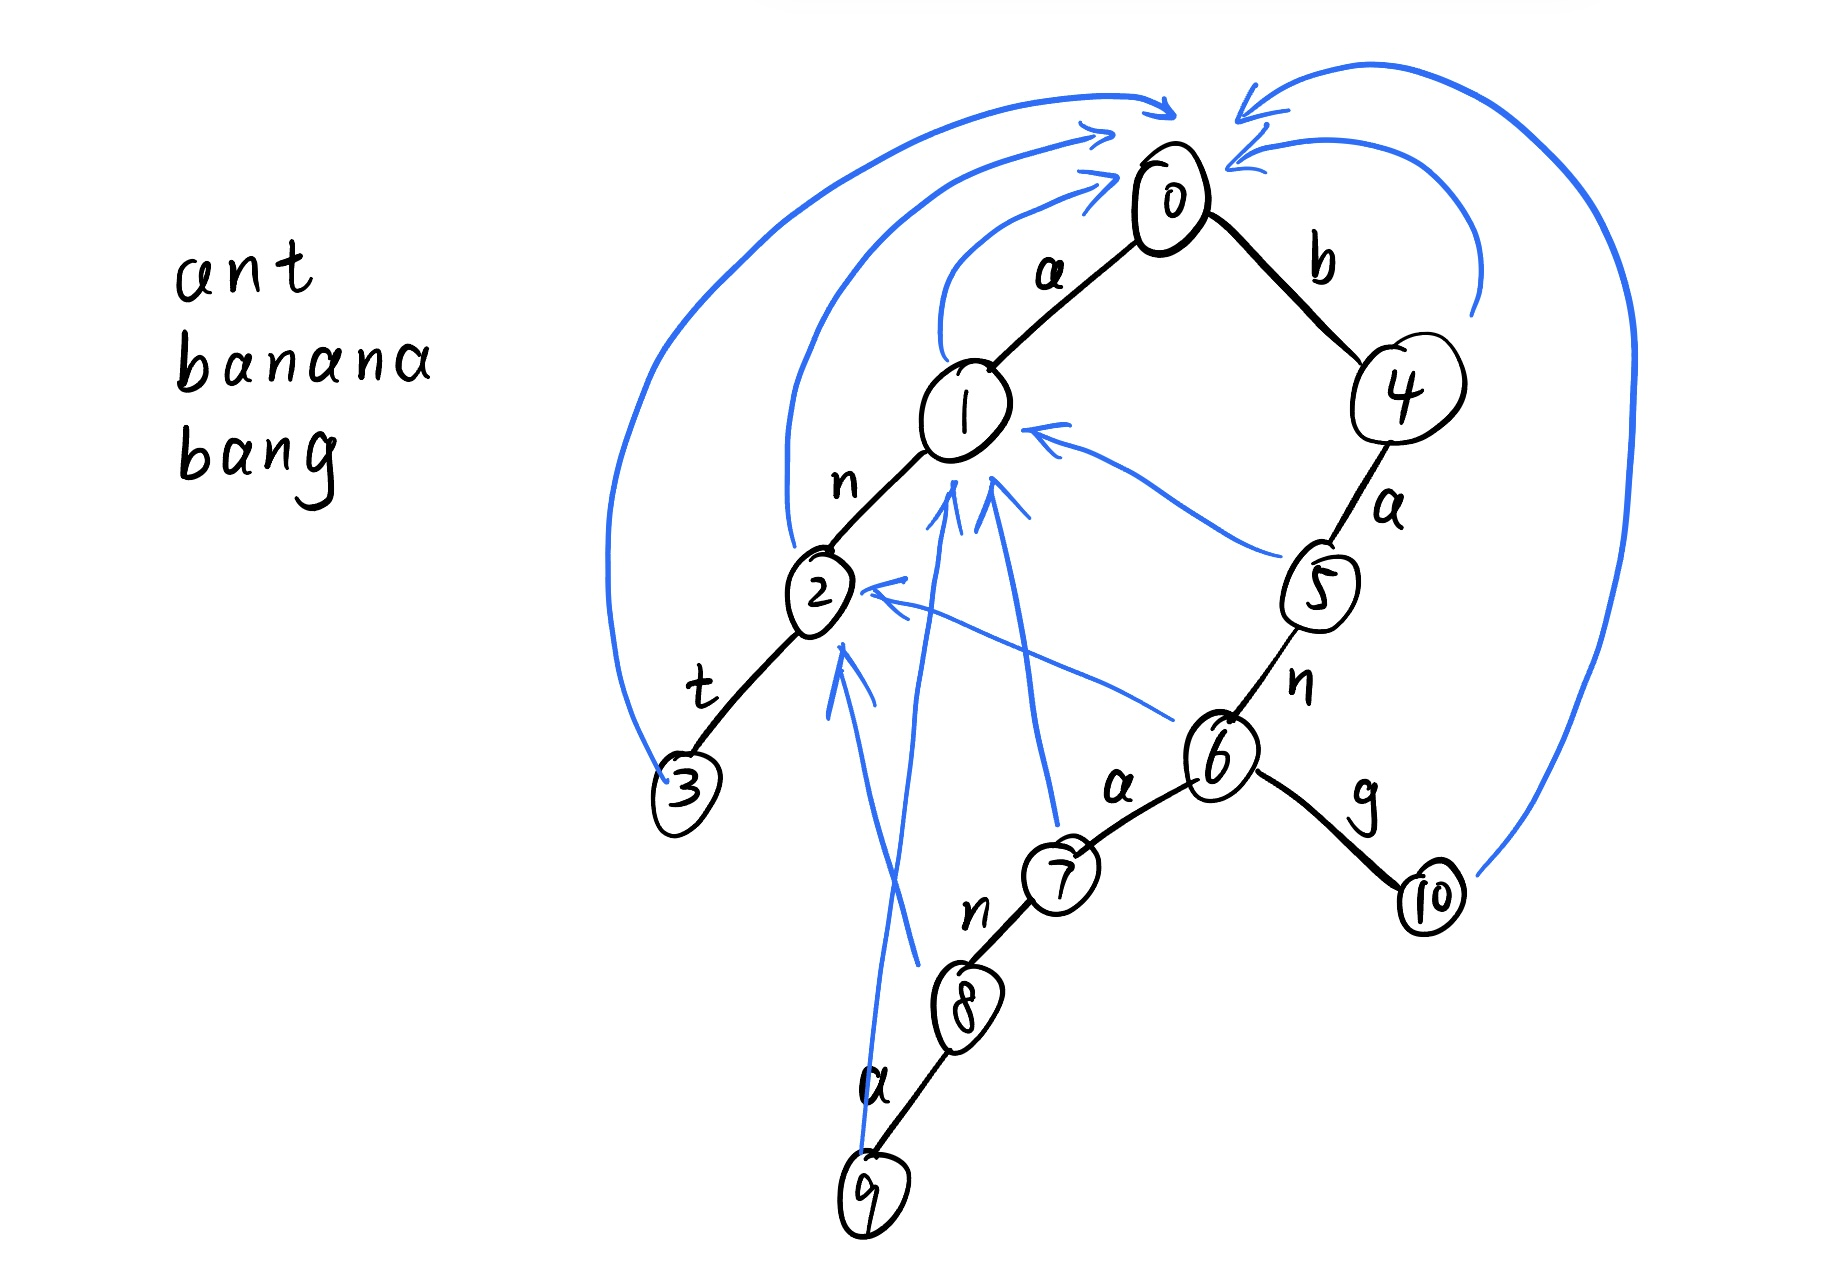
\includegraphics[width=0.8\textwidth]{pic/fail.jpg}
    \end{figure}

    \vspace{1em}\pause
    如果我们想找到所有 $\mathcal{F}(p)$ 中的节点,
    只需要沿着 fail 树一直往上跳即可。
\end{frame}

\begin{frame}[fragile]{求 fail}
    \small
    现在,我们来看如何求 \verb|fail| 数组。
    注意,必须先把所有模式串的字典树建立好,才能开始求 \verb|fail|。

    \vspace{1em}\pause
    我们用字典树的 BFS 序来求 \verb|fail|,现在遍历到节点 \verb|u|,我们
    来枚举它的下一个节点 \verb|v=ch[u][c]|。
    
    \vspace{1em}\pause
    试想,如果 \verb|fail[v]| 不指向根,那么 \verb|fail[v]=q|,其中 \verb|q=ch[f][c]|(一定存在这样的 $f$)。
    这个 \verb|f| 在哪里找?

    \vspace{1em}\pause
    显然,$f\in \mathcal{F}(u)$,因此只要从 $u$ 出发,沿着 fail 树往上跳,如果
    发现某个 \verb|f| 满足 \verb|ch[f][c]|$\neq 0$ 就立刻停止,并令 \verb|fail[v]=ch[f][c]|。
\end{frame}

\begin{frame}[fragile]{求 fail}
    \small
    \begin{lstlisting}[language=c++]
void getfail(){
    queue<int> q;
    for(int c = 0; c < 26; c++)
        if(ch[0][c]) q.push(ch[0][c]);
    while(!q.empty()){
        int u = q.front(); q.pop();
        for(int c = 0; c < 26; c++){
            int v = ch[u][c];
            if(!v) continue;
            int f = fail[u];
            while(f && !ch[f][c]) f = fail[f];
            fail[v] = ch[f][c];
            q.push(v);
        }
    }
}
    \end{lstlisting}

    它是 $O(n)$ 的,为什么?
\end{frame}

\begin{frame}[fragile]{[P3808] AC自动机(简单版)}
    \small
    给定 $n$ 个模式串 $s_i$ 和一个文本串 $t$,求有多少个不同的模式串在文本串里出现过。  

    两个模式串不同当且仅当他们 \textbf{编号} 不同。
\end{frame}

\begin{frame}[fragile]{[P3808] AC自动机(简单版)}
    \footnotesize

    首先构建模式串的字典树,并求出 fail 数组。

    \vspace{.7em}\pause
    现在,我们在字典树上从根节点出发,顺着文本串 $s$ 一步一步走,即
    \verb|u=0|,\verb|u=ch[u][s[1]]|,\verb|u=ch[u][s[2]]|,……
    (我们先假设不会碰到走不下去的情况)

    \vspace{.7em}\pause
    可以知道,在这个过程中,$S_u$ 都在 $s$ 中出现过;$S_p\;(p\in \mathcal{F}(u))$
    也都在 $s$ 中出现过;除此之外不会有其它的出现过。

    \vspace{.7em}\pause
    这就产生了一种做法:令 \verb|appear[u]| 表示 $S_u$ 是否在 $s$ 中出现过,
    $u$ 每走一步,就把 \verb|appear[u]| 标记成 \verb|true|;然后令 $f$ 从 $u$
    出发,沿着 fail 一直跳到根,把途径的 \verb|appear[f]| 都标记成 \verb|true|.

    \vspace{.7em}\pause
    当然,在 $f$ 往上跳的过程中,如果发现 \verb|appear[f]| 已经被标记成了 \verb|true|,
    那么可以立即终止循环,因为之后的肯定早就被标记过了。这样可以保证
    fail 树上的每个节点只被标记一次,从而保证复杂度线性。

    \vspace{.7em}\pause
    现在,如果 $u$ 在走的过程中发现走不下去,怎么办?

    \vspace{.7em}\pause
    沿着 fail 往上跳,直到 \verb|ch[u][s[i]]|$\neq 0$ 为止。
    (请思考:为什么这样能保证不重不漏地标记在 $s$ 中出现过的所有 $S_p$)
\end{frame}

\begin{frame}[fragile]{[P3808] AC自动机(简单版)}
    \small
    代码像这样:

    \begin{lstlisting}[language=c++]
void traval(char s[]){
    int n = strlen(s+1), u = 0;
    for(int i = 1; i <= n; i++){
        int c = s[i] - 'a';
        while(u && !ch[u][c]) u = fail[u];
        u = ch[u][c];
        appear[u] = true;
        int f = fail[u];
        while(f && !appear[f])
            appear[f] = true, f = fail[f];
    }
}
    \end{lstlisting}

    \vspace{1em}\pause
    在字典树 insert 的过程中,记录一下每一个模式串 $t_i$ 对应的节点是哪个,
    记作 \verb|idx[i]|,然后根据 \verb|appear[idx[i]]| 来统计答案。
\end{frame}

\begin{frame}[fragile]{求 fail(路径压缩版)}
    \small
    我们可以在求 fail 的时候顺便压缩路径。

    \vspace{1em}\pause
    具体而言,因为我们知道在 traval 的过程中,
    如果发现 \verb|ch[u][c]=0|,我们会从 $u$ 出发沿着 fail 往上跳,
    直到找到 \verb|ch[f][c]=q|$\neq 0$ 的位置为止。
    我们不妨在求 fail 的时候就把这一步做好,一步到位令 \verb|ch[u][c]=q|.

    \pause
    \begin{lstlisting}[language=c++]
void getfail(){
    queue<int> q;
    for(int c = 0; c < 26; c++)
        if(ch[0][c]) q.push(ch[0][c]);
    while(!q.empty()){
        int u = q.front(); q.pop();
        int f = fail[u];
        for(int c = 0; c < 26; c++){
            int& v = ch[u][c];
            if(!v) v = ch[f][c];
            else fail[v] = ch[f][c], q.push(v);
        }
    }
}
    \end{lstlisting}
\end{frame}

\begin{frame}[fragile]{搜索(路径压缩版)}
    \small
    有了路径压缩,我们在 travel 的过程中就不需要跳 fail 了。
    (当然,标记答案的时候还是要跳 fail)

    \begin{lstlisting}[language=c++]
void traval(char s[]){
    int n = strlen(s+1), u = 0;
    for(int i = 1; i <= n; i++){
        int c = s[i] - 'a';
        u = ch[u][c];
        appear[u] = true;
        int f = fail[u];
        while(f && !appear[f])
            appear[f] = true, f = fail[f];
    }
}
    \end{lstlisting}

    以后我们都用路径压缩的版本。
\end{frame}

\begin{frame}[fragile]{[P5357] 【模板】AC自动机}
    \small
    给定 $n$ 个模式串 $s_i$ 和一个文本串 $t$,求每个模式串在文本串里出现的次数。  
\end{frame}

\begin{frame}[fragile]{[P5357] 【模板】AC自动机}
    \footnotesize
    我们回顾之前的 travel 代码,很容易会想把 \verb|appear| 数组改成
    \verb|cnt| 数组,用于统计出现次数,像这样:

    \begin{lstlisting}[language=c++]
void traval(char s[]){
    int n = strlen(s+1), u = 0;
    for(int i = 1; i <= n; i++){
        int c = s[i] - 'a';
        u = ch[u][c];
        cnt[u]++;
        int f = fail[u];
        while(f) cnt[f]++, f = fail[f];
    }
}
    \end{lstlisting}
    \pause

    但是,回顾我们之前说的,我们是如何保证 travel 的复杂度是线性的?

    \vspace{.7em}\pause
    必须要保证每个节点只被标记一次。可是这里我们不能保证,怎么办?
\end{frame}

\begin{frame}[fragile]{[P5357] 【模板】AC自动机}
    \footnotesize
    还记得 fail 构成一棵树吗?我们可以在 travel 的时候只令 \verb|cnt[u]++|,
    最后来一次 dfs,把每个节点 $u$ 的子树里面的 \verb|cnt| 全加起来。
    最后代码像这样:

    \begin{lstlisting}[language=c++]
void traval(char s[]){
    int n = strlen(s+1), u = 0;
    for(int i = 1; i <= n; i++){
        int c = s[i] - 'a';
        u = ch[u][c];
        cnt[u]++;
    }
}

void dfs(int u){
    for(int v : g[u])
        dfs(v), cnt[u] += cnt[v];
}
    \end{lstlisting}

    \pause
    当然,在调用完 travel 之后,要把 fail 树像存图那样存起来,
    然后再调用 dfs。
\end{frame}

\begin{frame}[fragile]{[SCOI2012] 喵星球上的点名}
    \footnotesize
    给定 $n$ 个文本串,$m$ 个模式串。
    如果模式串 $T_i$ 是文本串 $S_j$ 的子串,则 $S_j$ 对 $T_i$ 产生 $1$ 的贡献。

    \vspace{1em}
    求每个文本串对几个模式串产生了贡献、每个模式串得到了几个文本串的贡献。

    \vspace{1em}
    模式串、文本串总长均不超过 $10^5$,\textbf{字符集大小为} $10^4$。
\end{frame}

\begin{frame}[fragile]{[SCOI2012] 喵星球上的点名}
    \footnotesize
    统计贡献和模板题(简单版)没啥区别,主要说一下字符集大小为 $10^4$ 怎么办。

    \vspace{1em}\pause
    肯定不能开一个 \verb|ch[100010][10010]|,会 MLE。
    可以用 \verb|map|,不过个人建议用 \verb|unordered_map|:
    \begin{lstlisting}[language=c++]
unordered_map<int,int> ch[100010];
    \end{lstlisting}

    \vspace{1em}\pause
    这时候我们不能写路径压缩了,要回归朴素写法。判断 $u$ 是否存在下一个字符 $c$
    要用 \verb|ch[u].count(c)| 来判断。
\end{frame}

\begin{frame}[fragile]{[HNOI2006] 最短母串问题}
    \footnotesize
    给定  $n\;(\leq 12)$ 个字符串  $(S_1,S_2,...,S_n)$,长度均 $\leq 50$,
    要求找到一个最短的字符串  $T$,
    使得这  $n$ 个字符串  $(S_1,S_2,...,S_n)$ 都是  $T$ 的子串。
\end{frame}

\begin{frame}[fragile]{[HNOI2006] 最短母串问题}
    \footnotesize
    对于一个节点 $u$,如果它对应的串是一个模式串,我们就称它为“关键点”。

    \vspace{.7em}
    如果有一个串在 travel 过程中可以经过所有关键点,
    那么所有的模式串都是它的子串。

    \vspace{.7em}
    找一个最短的、在 travel 过程中可以经过所有关键点的串。

    \vspace{.7em}\pause
    我们令第 $i$ 个模式串对应的关键点权值为 $2^{i-1}$,非关键点权值为 $0$,
    我们在 travel 的过程中,把经过的点的权值或起来,
    最后达到 $2^n-1$ 时,就经过了所有关键点。

    \vspace{.7em}\pause
    出于 “最短” 考虑,我们可以 bfs,令当前串为 $T$,当前 travel 到的节点为 $u$,
    当前权值或为 $st$,记为状态 $(T,u,st)$。
    \pause 如果存在另一个状态 $(T',u,st)$ 且 $|T'|<|T|$,
    那么状态 $(T,u,st)$ 就是没用的。
    \pause 所以我们可以用一个数组 \verb|vis[u][st]|,
    当状态 $(*,u,st)$ 第一次产生时,就令 \verb|vis[u][st]=true|,
    下一次再到达 $(*,u,st)$ 时,根据 bfs 的性质,此时的串肯定比第一次时的串更长,
    因此这一次的状态是没用的,可以剪掉。

    \vspace{.7em}\pause
    由于每一对 $(u,st)$ 只会被访问一次,所以复杂度是 $O(nL\cdot 2^n)$. 
    题目要求输出方案,所以在 bfs 的过程中还要做一些额外的标记,请自己尝试完成。
\end{frame}

\begin{frame}[fragile]{[HNOI2004] L语言}
    \footnotesize
    标点符号的出现晚于文字的出现,所以以前的语言都是没有标点的。现在你要处理的就是一段没有标点的文章。  

    \vspace{1em}
    一段文章 $T$ 是由若干小写字母构成。一个单词 $W$ 也是由若干小写字母构成。一个字典 $D$ 是若干个单词的集合。我们称一段文章 $T$ 在某个字典 $D$ 下是可以被理解的,是指如果文章 $T$ 可以被分成若干部分,且每一个部分都是字典 $D$ 中的单词。  
    
    \vspace{1em}
    例如字典 $D$ 中包括单词 $\texttt{is},\texttt{name},\texttt{what},\texttt{your}$,则文章 $\texttt{whatisyourname}$ 是在字典 $D$ 下可以被理解的,因为它可以分成 $4$ 个单词:$\texttt{what},\texttt{is},\texttt{your},\texttt{name}$,且每个单词都属于字典 $D$,而文章 $\texttt{whatisyouname}$ 在字典 $D$ 下不能被理解,但可以在字典 $D'=D\cup\{\texttt{you}\}$ 下被理解。这段文章的一个前缀 $\texttt{whatis}$,也可以在字典 $D$ 下被理解,而且是在字典 $D$ 下能够被理解的最长的前缀。  
    
    \vspace{1em}
    给定一个字典 $D$,你的程序需要判断若干段文章在字典 $D$ 下是否能够被理解。并给出其在字典 $D$ 下能够被理解的最长前缀的位置。

    \vspace{1em}
    数据范围:字典里最多 $20$ 个单词,每个单词长度 $\leq 20$,文章长度 $\leq 2\times10^6$.
\end{frame}

\begin{frame}[fragile]{[HNOI2004] L语言}
    \footnotesize

    设 $f_i$ 表示 $T[1,i]$ 能否由字典中的单词拼接而成。\pause 
    现在开始 travel,设到达 $T[i]$ 时,节点编号为 $u$,那么
    \begin{equation*}
        f_i=\text{or}\; f_j,\quad j=i-|S_p|,\; \text{其中} p\in \mathcal{F}(u),\; \text{且} S_p\in D.
    \end{equation*}

    这样就得到了一种跳 fail 转移的做法,复杂度 $O(m \cdot |T| \cdot |s|)$,卡不过去。

    \vspace{1em}\pause
    注意到题目有一个特殊性质:单词长度 $\leq 20$.
\end{frame}

\begin{frame}[fragile]{[HNOI2004] L语言}
    \footnotesize

    维护一个 21 位二进制数 \verb|status|,表示 $T[i]$ 往前几位是可以的划分点。
    举例而言,如果 $T[1,i-1],T[1,i-5],T[1,i-9]$ 是可以被字典理解的,那么
    
    \verb|status = 00000 00000 01000 10001|

    \vspace{1em}\pause
    我们对每一个节点 $u$ 也维护一个二进制数 \verb|g[u]|,表示 $u$ 沿着 fail 树一直往上跳
    可以经过哪些\textbf{字典中的单词}的长度(我们认为空串也是字典中的单词)。

    \vspace{1em}
    举例而言,如果 $|S_u|=17$, $|S_{fail[u]}|=5$, $|S_{fail[fail[u]]}|=3$, 
    $fail[fail[fail[u]]]=0$,但是 $S_{fail[fail[u]]}\notin D$,
    那么

    \verb|g[u] = 00010 00000 00000 10000|

    \vspace{1em}\pause
    如果 travel 过程中,处理到 $T[i]$ 时位于节点 $u$,
    此时只要 \verb|status| 和 \verb|g[u]| 有相同的一位为 $1$,
    那么 $T[1,i]$ 就是可以被字典理解的。

    \vspace{1em}\pause
    例如在上述例子中,它们从右往左第 5 位均为 $1$,对应的情况
    就是 $T[1,i-5]$ 可以被字典理解,同时字典中恰好有一个长为 $5$ 的单词等于 $T[i-4,i]$,
    因此 $T[1,i]$ 可以被字典理解。
\end{frame}

\begin{frame}[fragile]{[HNOI2004] L语言}
    \footnotesize

    求 \verb|g[u]| 的过程可以写在 \verb|getfail| 里面,像这样:

    \begin{lstlisting}[language=c++]
void getfail(){
    queue<int> q;
    for(int c = 0; c < 26; c++){
        int v = ch[0][c];
        if(v){
            q.push(v);
            if(len[v]) g[v] = 1<<len[v]-1;
        }
    }
    while(!q.empty()){
        int u = q.front(); q.pop();
        int f = fail[u];
        for(int c = 0; c < 26; c++){
            int& v = ch[u][c];
            if(!v) v = ch[f][c];
            else{
                fail[v] = ch[f][c];
                g[v] = g[fail[v]];
                if(len[v]) g[v] |= (1<<len[v]-1);
                q.push(v);
            }
        }
    }
}
    \end{lstlisting}

    其中 \verb|len[u]| 在 $S_u\in D$ 时等于 $|S_u|$,在 $S_u\notin D$ 时等于 $0$.
\end{frame}

\begin{frame}[fragile]{[HNOI2004] L语言}
    \footnotesize

    最后 travel 的过程就像这样:

    \begin{lstlisting}[language=c++]
int traval(char s[]){
    unsigned status = 1;
    int n = strlen(s+1), u = 0, ans = 0;
    for(int i = 1; i <= n; i++){
        int c = s[i] - 'a';
        u = ch[u][c];
        if(status & g[u]) status = status<<1|1, ans = i;
        else status <<= 1;
    }
    return ans;
}
    \end{lstlisting}
\end{frame}

\begin{frame}{[JSOI2009] 有趣的游戏}
    \footnotesize

    小阳阳发明了一个有趣的游戏:有 $n$ 个玩家,每个玩家都有一个长度为 $l$ 的字母序列,任何两个玩家的字母序列不同。共有 $m$ 种不同的字母,所有的字母序列都由这 $m$ 种字母构成。为了方便,我们取大写字母的前 $m$ 个字母。   
    
    \vspace{1em}
    例如 $m=3,l=4,\texttt{ABAA}$ 和 $\texttt{CBCA}$ 是两个合法的字母序列。       
    
    \vspace{1em}
    现在由小阳阳来操控一台神奇的机器,每个时刻机器会随机产生一个字母,其中第 $i$ 种字母随机出来的概率为 $\dfrac{p_i}{q_i}$ ,显然 $\sum \limits_{k=1}^m \dfrac{p_i}{q_i}=1$。  
    
    \vspace{1em}
    这样 $T$ 个时刻后机器会产生一个长度为 $T$ 的字母序列。  
    
    \vspace{1em}
    如果某个时刻某个玩家发现自己的字母序列在机器产生的字母序列中出现了,“出现”的定义是玩家的字母序列是机器产生的字母序列中连续的一段,那么我们称这个玩家获胜,游戏结束。       
    
    \vspace{1em}
    现在小阳阳感兴趣的一个问题是,每个玩家分别有多大的概率能获得这场游戏的胜利呢?

    \vspace{1em}
    数据范围:$n,l,m\leq 10$.
\end{frame}

\begin{frame}[fragile]{[JSOI2009] 有趣的游戏}
    \footnotesize

    构造一个路径压缩版的AC自动机,问题转化为:从根节点出发,每次按某种概率随机
    跳入下一个点,当跳到的节点恰好对应某个玩家的串时,游戏停止,该玩家获胜。
    
    \vspace{1em}\pause
    假如当前在 $u$ 节点,
    那么添加一个字母 $i$ 的概率是 $\frac{p_i}{q_i}$,因此
    下一步走到 $v$ 的概率是
    \begin{equation*}
        P_{u,v}=\sum_{1\leq i\leq m,\; ch[u][i]=v} \frac{p_i}{q_i}.
    \end{equation*}

    \vspace{1em}\pause
    特别地,如果 $u$ 恰好对应某个玩家的串,那么就没有下一步了;换言之,以后会一直停在 $u$。所以
    \begin{equation*}
        P_{u,u}=1,\;P_{u,v}=0(v\neq u),\quad \text{若} u \text{恰好对应某个玩家的串}
    \end{equation*}

    \vspace{1em}\pause
    现在,把 $P$ 当成一个矩阵,$P^k_{u,v}$ 就表示从节点 $u$ 出发,经过 $k$ 步后到达节点 $v$ 的概率。
    显然我们要求的就是 $P^\infty_{0,p_i}$ ($p_i$ 是第 $i$ 个玩家的串对应的节点)。
    
    \vspace{1em}\pause
    因为题目要求保留两位小数输出,并非精确输出,我们可以用很大的数来代替 $\infty$。
    例如可以取 $\infty=2^50$,这样只要重复做 50 次 \verb|P=P*P| 即可。
\end{frame}

\begin{frame}[fragile]{[COCI2015] Divljak}
    \footnotesize

    Alice 有 $n$ 个字符串 ${S}_1, {S}_2, \ldots, {S}_n$,Bob 有一个字符串集合 ${T}$,一开始集合是空的。
    接下来会发生 $q$ 个操作,操作有两种形式:

    \begin{enumerate}
        \item \verb|1 P|:Bob 往自己的集合里添加了一个字符串 ${P}$。
        \item \verb|2 x|:Alice 询问 Bob,集合 ${T}$ 中有多少个字符串包含串 ${S}_x$
        (我们称串 ${A}$ 包含串 ${B}$,当且仅当 ${B}$ 是 ${A}$ 的子串)。
    \end{enumerate}

    \vspace{1em}
    对于 $100\%$ 的数据,$1 \leq n,q \leq 10^5$,字符串由小写字母构成,$S$ 和 $P$ 的总长分别 $\le 2 \times 10^6$。
\end{frame}

\begin{frame}[fragile]{[COCI2015] Divljak}
    \footnotesize

    先对 Alice 的所有串建立AC自动机。现在考虑 Bob 添加一个字符串 $P$。

    \vspace{1em}\pause
    设 $P$ 在 travel 的过程中依次经过节点 $u_1,...,u_k$,那么在AC自动机上,
    $P$ 包含的所有串就是 $\mathcal{F}(u_1)\cup\cdot\cup \mathcal{F}(u_k)$.
    我们希望对这些点都进行 $+1$ 操作,然后对于 Alice 的询问,直接输出 $S_x$ 对应节点的权值即可。

    \vspace{1em}\pause
    首先对 fail 数组建立树结构(下面的 dfs 序、lca,均指 fail 树,而不是字典树)。
    将 $u_1,...,u_k$ 按 dfs 序排序,并去重。
    现在用树上差分的思想,对 $u_1,...,u_k$ 打上 $+1$ 标记,再对 $lca(u_1,u_2), lca(u_2,u_3),..., lca(u_{k-1},u_k)$
    打上 $-1$ 标记。然后如果想知道一个点 $x$ 的权值,只要把 $x$ 子树里的所有标记加起来即可(子树对应 dfs 序里的一个区间)。

    \vspace{1em}\pause
    单点标记、区间求和,可以用树状数组完成。求 lca 需要倍增(或者树链剖分)。
\end{frame}

\begin{frame}[fragile]{[NOI2011] 阿狸的打字机}
    \footnotesize    
    阿狸喜欢收藏各种稀奇古怪的东西,最近他淘到一台老式的打字机。打字机上只有 $28$ 个按键,
    分别印有 $26$ 个小写英文字母和 `B`、`P` 两个字母。经阿狸研究发现,这个打字机是这样工作的:
    \begin{itemize}
        \item 输入小写字母,这个字母会加在凹槽的最后。
        \item 按一下印有 \verb|B| 的按键,打字机凹槽中最后一个字母会消失。
        \item 按一下印有 \verb|P| 的按键,打字机会在纸上打印出凹槽中现有的所有字母并换行,但凹槽中的字母不会消失。
    \end{itemize}
    例如,阿狸输入 \verb|aPaPBbP|,纸上被打印的字符如下:
\begin{lstlisting}
a
aa
ab
\end{lstlisting}
    我们把纸上打印出来的字符串从 $1$ 开始顺序编号,一直到 $n$。打字机有一个非常有趣的功能,
    在打字机中暗藏一个带数字的小键盘,在小键盘上输入两个数 $(x,y)$(其中 $1\leq x,y\leq n$),
    打字机会显示第 $x$ 个打印的字符串在第 $y$ 个打印的字符串中出现了多少次。
    请你实现这个功能。

    \vspace{.5em}
    对于 $100\%$ 的数据,$1\leq n\leq 10^5$,$1\leq m\leq10^5$,第一行总长度 $\leq 10^5$。
\end{frame}

\begin{frame}[fragile]{[NOI2011] 阿狸的打字机}
    \footnotesize

    假设第 $y$ 个字符串在 travel 的过程中依次经过 $u_1,...,u_k$,
    我们对 $\mathcal{F}(u_1),...,\mathcal{F}(u_k)$ 分别执行 $+1$ 操作,
    那么现在任意一个点 $p$ 的权值就表示 $S_p$ 在第 $y$ 个字符串中出现了几次。
    (注意和上一题对比!)

    \vspace{1em}\pause
    同样用树上差分,我们对 $u_1,...,u_k$ 打上 $+1$ 标记,每一个点的权值就是
    它子树上所有标记之和。仍然用树状数组维护。

    \vspace{1em}\pause
    我们把所有询问按 $y$ 从小到大排序,然后模拟阿狸的打字过程。每打一个小写字母,
    就走一步,然后打上新的 $+1$ 标记;每打一个回格,就把当前点的 $+1$ 标记清除
    (即打上 $-1$ 标记);每打一个输出,就枚举 $y$ 为当前输出串的那些询问,
    求第 $x$ 个输出串对应节点的权值。
\end{frame}

\begin{frame}
    \begin{center}
        {\Huge\calligra Thank You}
    \end{center}
\end{frame}

\end{document}